\documentclass[11pt]{article}
\usepackage{graphicx}
\usepackage{amsmath,amsthm,amsfonts}
\usepackage{epsfig,graphics}
\usepackage{hyperref}
\usepackage{verbatim}
\usepackage{mathrsfs}
\usepackage{xcolor}

\setlength{\textheight}{8.5in}
\setlength{\evensidemargin}{0.0in}
\setlength{\oddsidemargin}{0.0in}
\setlength{\topmargin}{-0.5in}
\setlength{\textwidth}{6.5in}

\newtheorem{theorem}{Theorem}
\newtheorem*{theorem*}{Theorem}
\newtheorem{claim}{Claim}
\newtheorem*{claim*}{Claim}
\newtheorem{lemma}{Lemma}
\newtheorem*{lemma*}{Lemma}
\newtheorem{proposition}{Proposition}
\newtheorem*{proposition*}{proposition}
\newtheorem{exercise}{Exercise}
\newtheorem*{exercise*}{Exercise}
\newtheorem{corollary}{Corollary}
\theoremstyle{definition}
\newtheorem{definition}{Definition}
\newtheorem{fact}{Fact}
\newtheorem*{fact*}{Fact}



\newcommand{\handout}[6]{
   \renewcommand{\thepage}{#1-\arabic{page}}
   \noindent
   \begin{center}
      \vbox{
    \hbox to \textwidth { #2 \hfill #3 }
       \vspace{4mm}
       \hbox to \textwidth { {\Large \hfill #4  \hfill} }
       \vspace{2mm}
       \hbox to \textwidth { { #5 \hfill #6} }
      }
   \hrulefill
   \end{center}
   \vspace*{4mm}
}

%\newcommand{\lecture}[5]{\handout{#1}{#2}{#3}{#4}{#5}}


% Types of Variables
\newcommand{\bvar}[1]{\mathbf{#1}} % bold variable
\newcommand{\mvar}[1]{\bvar{#1}} % matrix variable
\newcommand{\vvar}[1]{\vec{#1}} % vector variable

% Domains
\newcommand{\R}{\mathbb{R}}
\newcommand{\Z}{\mathbb{Z}}
\newcommand{\redgevec}{\R^{E}}
\newcommand{\rvertvec}{\R^{V}}
\newcommand{\rPos}{\R^{+}}
\newcommand{\rNonNeg}{\R^{\geq 0}}

% Symbol for definitions
\newcommand{\defeq}{\stackrel{\mathrm{\scriptscriptstyle def}}{=}}

% Optimization
\DeclareMathOperator*{\argmin}{arg\,min}
\DeclareMathOperator{\Cone}{Cone}
\DeclareMathOperator{\Cut}{CUT}

% Types of Graphs
\newcommand{\nlap}{\mathscr{L}_G}
\newcommand{\pseudo}[1]{{#1}^\dagger}
\newcommand{\lapPseudo}{\pseudo{\lap}}
\newcommand{\adj}{A}
\newcommand{\incMatrix}{\mvar{B}}
\newcommand{\diag}{\operatorname{diag}}
\newcommand{\rMatrix}{\mvar{R}} % resistance matrix
\newcommand{\iMatrix}{\mvar{I}} % identity matrix
\newcommand{\Vol}{\textrm{Vol}}


% Vectors
\newcommand{\1}{\vec{1}}
\renewcommand{\dot}[1]{\langle {#1} \rangle}

%other
\DeclareMathOperator{\sgn}{sgn}


\usepackage[symbol]{footmisc}
\usepackage{color}
\renewcommand{\thefootnote}{\fnsymbol{footnote}}
\begin{document}

\handout{}{CS 591 O1: Iterative Methods for Graph Algorithms and Network Analysis}{Fall 2018}{Lecture 3: More on Averaging and Random Walks Processes}{Instructor: Lorenzo Orecchia}{Scribe: Erasmo Tani}

\section{Random Walks and Averaging Processes}
Last time we discussed two different processes related to the adjacency matrix of a graph. The first process is the \textbf{random walk process} described by the random walk operator $W = AD^{-1}$ which is the transition matrix of the natural random walk over the vertices of $G$. The second process is the \textbf{averaging process} by means of which the vertices of the graph, assigned an initial belief value, try to reach a global consensus by repeating a local step. This second process corresponds to the operator $\frac{1}{2}(I + W^T) = \frac{1}{2}(I+D^{-1}A)$\\

\noindent
In the random walk process we work with probability vectors $p \in \R^V$ representing the probability of being at a particular vertex at a specific time. In the averaging process we work with $x$ vectors that represent the amount of mass on the arcs (/ edges). Recall that these two representations are related by:
\begin{equation}\label{change_of_basis}
    \boxed{p = Dx}
\end{equation}

\noindent
The random walk process converges to the standard random walk stationary distribution $\pi$ where $\pi \in \Delta_n$ and for any vertex $i \in V$: $\pi_i \sim d_i$ where $d_i$ denotes the degree of $i$ in $G$. On the other hand, the second process converges to: 
\[
    \bar{x} = \frac{\sum_i d_i x_i}{vol(G)}\vec{1}
\]

\noindent
One can check that the averaging process does, in fact, correspond to having each vertex compute the average of its neighbours:

\[
    \left(\frac{1}{2}(I + W^T)x\right)_i = \frac{1}{2}\left(x_i + \frac{1}{d_i}\sum_{j \sim i} x_j\right).
\]

\noindent
In particular, the action of $W^T$ corresponds to the averaging the value of every neighbour (Figure \ref{fig:Wt}), and $\frac{1}{2}(I+W^T)$ simply averages the result with the current value.

\begin{figure}[h]
    \centering
    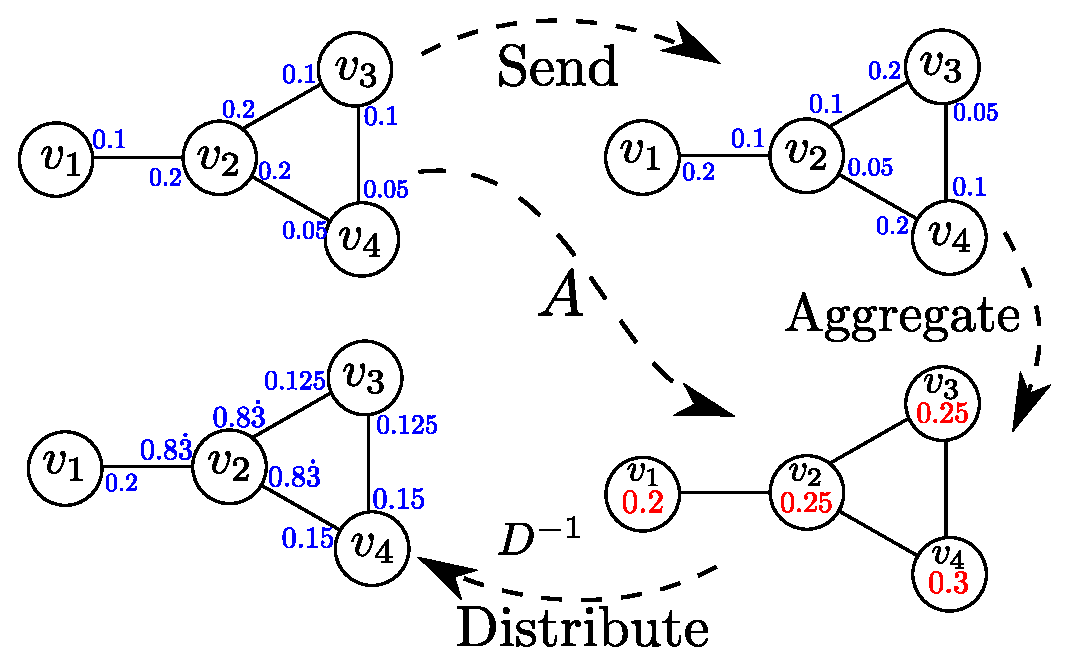
\includegraphics[scale=0.65]{WT.eps}
    \caption{The action of $W^T$ on the vector $x = ({\color{blue}0.1},{\color{blue}0.6},{\color{blue}0.2},{\color{blue}0.1})$.}
    \label{fig:Wt}
\end{figure}

\section{Hilbert Space Interpretation}
One can think of the $x$ vectors as living in the Hilbert space with inner product $\langle\cdot ,\cdot\rangle_D: \R^V \to \R$ given by:
\[
    \langle x,y \rangle_D = x^TDy
\]
And similarly the $p$ vectors live in the dual space with inner product: $\langle \cdot,\cdot\rangle_{D^{-1}}: \R^V \to \R$ given by:
\[
    \langle p,q \rangle_{D^{-1}} = p^TD^{-1}q
\]
for any $x$ the corresponding vector $p$ will equal $\Phi(x)$ where $\Phi$ is the isomorphism guaranteed by the Riesz representation theorem\footnote{Read more about it: \url{https://en.wikipedia.org/wiki/Riesz_representation_theorem}}.

\begin{figure}[h]
    \centering
    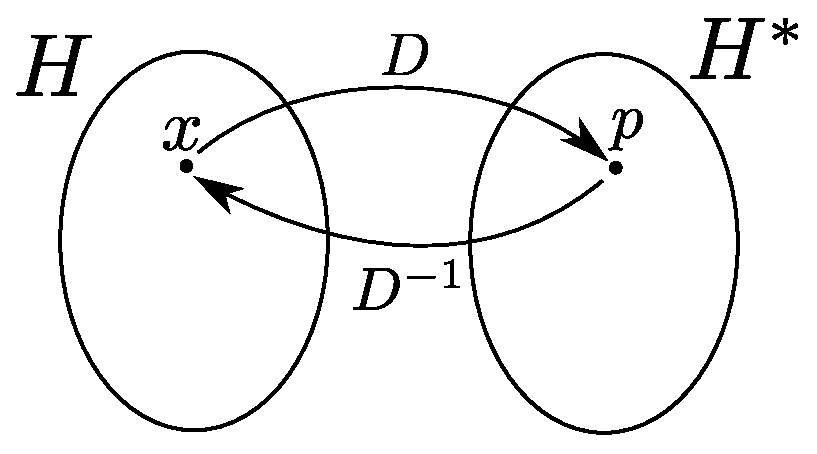
\includegraphics[scale=.75]{HSpaceSGT.eps}
    \caption{Vertex probability vectors $p$ live in the dual Hilbert space to that of edge mass vectors $x$.}
    \label{fig:my_label}
\end{figure}

\section{Measuring Convergence to the Fixed Point}
An important choice to make when tracking the dynamics of these processes, is the choice of potential function: how do we measure distance from the fixed point?\\

\noindent
In the \textbf{averaging process} it makes sense to track the distance of a mass assignment $x$ from the optimum by:
\[
    \phi_{avg}(x):= \sum_{i\in V} \pi_i \left(x_i - (\sum_{j \in V} \pi_j x_j)\right)^2 = Var_{i \sim \pi}(x_i)
\]

\noindent
By applying the conversion in $(\ref{change_of_basis})$ we see that this corresponds to:

\[
    \phi_{avg}(x) = ||x - \bar{x}||_{\pi}^2 = ||D^{-1}p - \bar{x} D^{-1}\vec{1} ||^2_D = ||p - \bar{x}\vec{1}||^2_{D^{-1}} = ||p-\pi||^2_{D^{-1}}
\]
\textcolor{blue}{edit:
\[
    \phi_{avg}(x) = ||x - (\pi^T x)\vec{1}||_{\pi}^2 = \frac{1}{vol(G)}||D^{-1}p - \frac{1}{vol(G)}\vec{1} ||^2_D = \frac{1}{vol(G)}||p - \frac{1}{vol(G)}D\vec{1}||^2_{D^{-1}} = \frac{1}{vol(G)}||p-\pi||^2_{D^{-1}}
\]}

which corresponds naturally to a way to measure distance from the optimum in the \textbf{random walk} process.

\section{Why Laplacians?}
The above analysis can provide motivation for the use of Laplacian matrices to study graph algorithms. One can in fact prove the following claim:
\begin{claim}
The potential function defined above is the quadratic form of the Laplacian of a suitably defined graph. I.e there exists some graph $H$ such that, for all $x \in \R^V$:
$\phi_{avg}(x) = x^TL(H)x$.
\end{claim}
\begin{proof}
One can define a graph $K_G$ as follows: $V(K_G) = V(G)= V$ and $E(K_G) = \binom{V}{2}$, so that the graph is complete, with weigths $w_{K_G}(ij) = \frac{d_id_j}{vol(G)}$~\footnote[1]{Recall that for any $S \subset V$: $vol(S):= \sum_{i \in S} d_i$ and $vol(G):= vol(V)$.}\\

\end{proof}

\noindent
We also observe that the value of the quadratic form $x^TL(G)x$ defined by the Laplacian matrix of $G$ measures the rate of convergence towards the stationary distribution at $x$. In fact, consider the continuous version of the averaging process given by:

\[
    \frac{dx(t)}{dt} = - (I-W^T)x(t)
\]


\noindent
We have:
\begin{align*}
    \frac{d}{dt}\left(||x - \bar{x}||_D^2\right) &= \left(\frac{d}{dt}x(t)\right)^TD(x(t)-\bar{x})\\
    &= \left(-(I-W^T)x(t)\right)^TD(x(t)-\bar{x})\\
    &= -x(t) (D-A)(x-\bar{x}) = -x^T(D-A)x
\end{align*}

\textcolor{blue}{edit:
\begin{align*}
    \frac{1}{2}\frac{d}{dt}\left(||x - \bar{x}||_D^2\right) &= \left(\frac{d}{dt}x(t)\right)^TD(x(t)-\bar{x})\\
    &= \left(-(I-W^T)x(t)\right)^TD(x(t)-\bar{x})\\
    &= -x(t) (D-A)(x-\bar{x}) = -x^T(D-A)x
\end{align*}}

\noindent
Where the last step above uses the fact that:
\[
    L\vec{1} = 0.
\]



\end{document}